\section{Method}
\label{sec:method}
\begin{figure}[t]
  \centering
  \vspace*{2mm}
  \subfloat[]{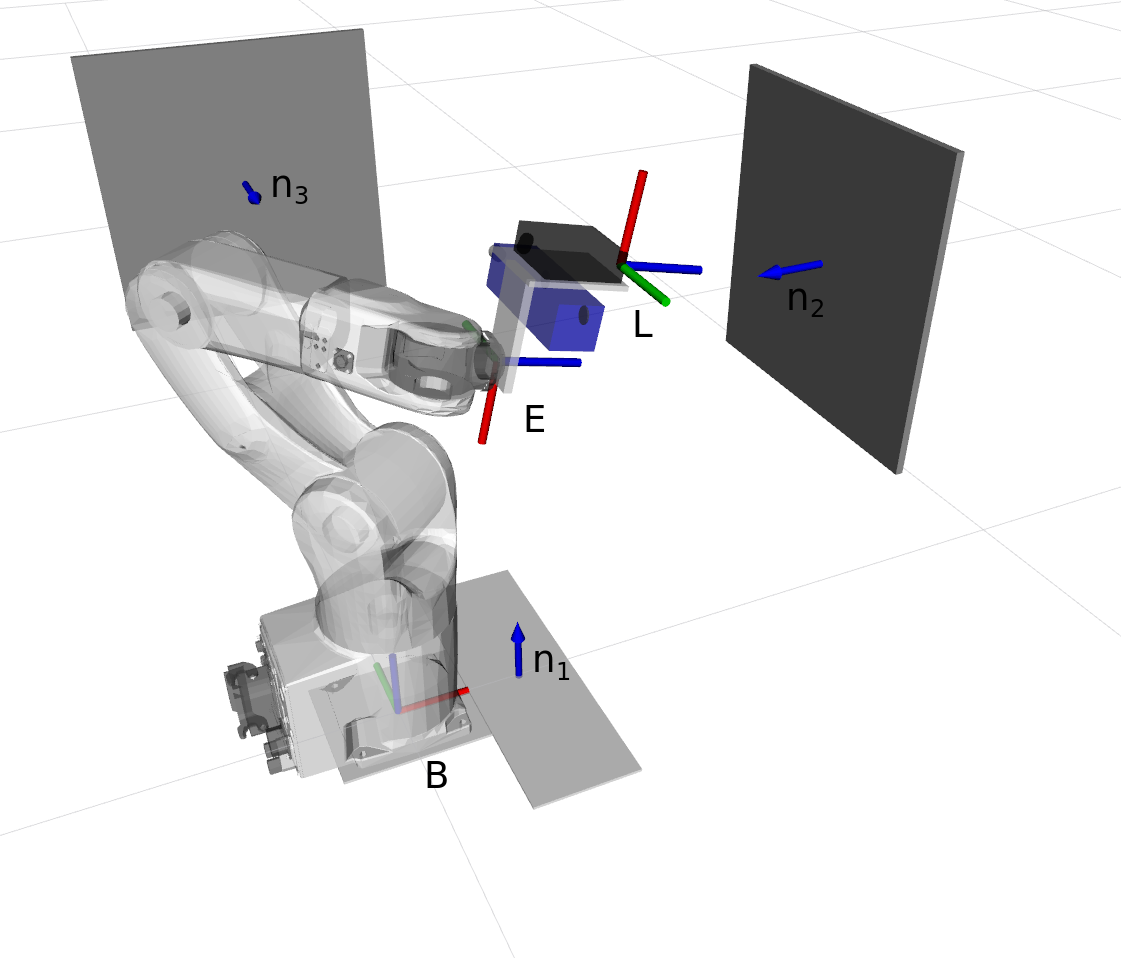
\includegraphics[height=60mm]{robot_setup}}
  \caption{Robot setup for the calibration}
  \label{fig:robot_setup}
\end{figure}

%TODO: draw a diagram which shows the frames from link0-link6, laser frame,and the frames on all the three planes%

The calibration setup is depicted in \fref{fig:robot_setup}, where three perpendicular planes ($k=1,2,3$) are installed around the robot. An \ac{lrf} is attached on the robot flange. For each plane, the robot is moved to $N$ poses such that the \ac{lrf} is directed to the respective plane. One data set from the \ac{lrf} consists of hundreds of data points, so $M$ data points are selected randomly from the \ac{lrf} data for each pose, together with the joint angles of the robot. 

This section provides the detail on how to calibrate both the extrinsic parameters of the LRF and the robot kinematics parameters. First, the initial estimate of the LRF extrinsic parameter is obtained by using the linear least-square method based on the data from one of the planes. After that, the LRF extrinsic parameters and the robot kinematics parameters are optimized simultaneously to satisfy the three planar constraints, by using the Levenberg Marquardt nonlinear optimization method. At the end of this section, we explain how we can use \ac{svd} to analyse which calibration parameters are identifiable, and the steps to handle the unidentifiable parameters are then presented. 
\subsection{Obtaining the Initial Estimate of the \ac{lrf} Extrinsic Parameters}
\label{sec:first_step}
To obtain an initial estimate of the \ac{lrf} extrinsic parameters, only the data from one plane is necessary. Arbitrarily, the bottom plane $plane 1$ is chosen. The extrinsic parameters of the \ac{lrf} $\vb*{{^E}T_L}$, i.e. the homogeneous transformation from the robot flange coordinate frame to the \ac{lrf} coordinate frame, is estimated by the following calculation. 

Let $p_i$ be one of the data points from the \ac{lrf} which lies on the $plane 1$, $n_1$ be the normal unit vector of $plane 1$, and $d_1$ be the perpendicular distance from the origin of the robot coordinate system to $plane 1$. The subscript/superscript B, E, and L denote the coordinate frame of the robot base, robot flange, and the \ac{lrf}, while the subscript i and j refer to the data point index and the robot pose index respectively. Since $p_1$ is located on the $plane 1$, it has to satisfy the following equation:
  \begin{equation}
  \label{eq:1}
  (\vb*{{^B}n_1}) ^T (\vb*{{^B}p_i}) - {^B}d_1 = 0
   \end{equation}
$\vb*{{^B}p_i}$ depends on the robot pose $\vb*{{^B}T_{E,j}}$ at pose index j and the \ac{lrf} extrinsic parameter $\vb*{{^E}T_L}$, so equation \ref{eq:1} can be expanded:
  \begin{equation}
  (\vb*{{^B}n_1}) ^T (\vb*{{^B}T_{E,j}}) (\vb*{{^E}T_L}) (\vb*{{^L}p_i}) - {^B}d_1 = 0
  \end{equation}
$\vb*{{^B}n_1}$ and $^{B}d_1$ are known approximately ($[0 \; 0\; 1\;0]$ and $0.0$), $\vb*{{^B}T_{E,j}}$ can be computed from the robot's joint angles at pose j, and $\vb*{{^L}p_i}$ is obtained from the laser. Let $\vb*{n^{'}_j} = (\vb*{{^B}n_1}) ^T (\vb*{{^B}T_{E,j}}) = 
\left[n^{'}_{j,1} \; n^{'}_{j,2} \; n^{'}_{j,3}  \; n^{'}_{j,4} \right]$, then  
  \begin{equation}
  \label{eq:3}
  (\vb*{n^{'}_j}) ^T (\vb*{{^E}T_L}) (\vb*{{^L}p_i}) - {^B}d_1 = 0
  \end{equation}
The only unknown in equation \ref{eq:3} is $\vb*{{^E}T_L}$ which has 12 elements $r_{uv}$, where u and v denote the column and the row index of the matrix. Note that the fourth row only consists of 0 and 1. 
Without any loss of generality, let's assume that the data points from the \ac{lrf} lies on the XZ planes in the laser frame $L$, so $\vb*{{^L}p_i} = \left[{^L}p_{i,x} \; 0 \; {^L}p_{i,z}\; 1\right]$. If we expand the equation above and rearrange such that the components of $\vb*{{^E}T_L}$ are gathered as a vector $\vb*{\Phi_L}$, we have
\begin{equation}
\label{eq:4}
  (\vb*{x_{ji}})  ^T (\vb*{\Phi_L}) = {^B}d_1 -  n^{'}_{j,4}
\end{equation}
where 
\begin{multline}
  \vb*{x_{ji}} = \left[{^L}p_{i,x}n^{'}_{j,1} \quad {^L}p_{i,x}n^{'}_{j,2}\quad {^L}p_{i,x}n^{'}_{j,3}\quad  {^L}p_{i,z}n^{'}_{j,1}\right. \\ 
\left. {^L}p_{i,z}n^{'}_{j,2}\quad {^L}p_{i,z}n^{'}_{j,3} \quad n^{'}_{j,1} \quad n^{'}_{j,2} \quad n^{'}_{j,3} \right]
\end{multline}, 
and
\begin{multline}
  \vb*{\Phi_L} = \left[r_{11} \quad r_{21} \quad r_{31} \quad r_{13} \quad r_{23} \quad r_{33} \quad r_{14} \quad r_{24}  \quad r_{34} \right] 
\end{multline}
For each data point i, we obtain such equation as in equation \ref{eq:4}. For $M$ data points per pose and a total of $N$ robot poses, we have $MN$ such equations. The equations can be stacked together to form the following matrix equation:
\begin{equation}
\label{eq:7}
  \vb*{X}   \vb*{\Phi_L} = \vb*{D}
\end{equation}
where 
\begin{equation}
X =\begin{bmatrix}
x_{11} \\ x_{12} \\ \cdots\\x_{1M}\\ x_{21}\\ \cdots\\ x_{2M} \\ \cdots \\ x_{NM}
\end{bmatrix} \;, \; D =\begin{bmatrix}
{^B}d_1 -  n^{'}_{1,4} \\ {^B}d_1 -  n^{'}_{1,4}  \\ \cdots\\ {^B}d_1 -  n^{'}_{1,4}  \\ {^B}d_1 -  n^{'}_{2,4} \\ \cdots\\ {^B}d_1 -  n^{'}_{2,4}  \\ \cdots \\{^B}d_1 -  n^{'}_{N,4} 
\end{bmatrix}
\end{equation}
Equation \ref{eq:7} can be solved by linear least square procedure to obtain $\vb*{\Phi_L}$. $\vb*{{^E}T_L}$ can then be computed as follows:
\begin{enumerate}
\item The parameters $[r_{11}, r_{21}, r_{31}]$ and $[r_{13}, r_{23}, r_{33}]$ are supposed to be unit vectors, so they should be normalized. They consistute the first and the third column of the matrix ${^E}T_L$
\item The parameters $[r_{14}, r_{24}, r_{34}]$ constitutes the position component of the matrix ${^E}T_L$, or its fourth column
\item The parameters $[r_{12}, r_{22}, r_{32}]$ can be calculated as the cross product of  $[r_{13}, r_{23}, r_{33}]$ and $[r_{11}, r_{21}, r_{31}]$ 
\end{enumerate}

To use the extrinsic parameters $\vb*{{^E}T_L}$ for the subsequent step, 9 parameters would be too redundant. Therefore, we choose the axis-angle representation for the rotation part of ${^E}T_L$ which gives us 4 parameters $[r_1, r_2, r_3, r_4]$, and 3 more parameters for the location part $[p_x, p_y, p_z]$. 


\subsection{Optimizing both the \ac{lrf} Extrinsic Parameters and Robot Kinematic Parameters}
\label{sec:second_step}
In the second step, the data from all the three planes are used to optimize the parameters of the \ac{lrf}, robot kinematics, as well as the plane parameters. The objective function is described as follows:

\begin{equation}
 \vb{f(\Phi)} =  \sum_{k=1}^{3} \sum_{j=1}^{N} \sum_{i=1}^{M} ((\vb*{{^B}n_1}) ^T (\vb*{{^B}p_i}) - \vb*{{^B}d_1})^2
\end{equation}

The parameters $\vb*{\Phi}$ consists of the followings:
\begin{enumerate}
\item Robot kinematics parameters. We choose the modified DH parameters *** $[a_i \;, \alpha_i \;,\theta_i \;,d_i], i=1, 2, \cdots ,6$ to represent the robot kinematics, so we have 6*4 = 24 DH parameters for a 6 \ac{dof} robot arm
\item Laser extrinsic parameters. As mentioned in the previous section, we use the axis angle representation for the rotation part $[r_1, r_2, r_3, r_4]$,and the location is represented by 3 numbers $[p_x, p_y, p_z]$. 
\item Plane parameters. Each plane has 4 parameters $[n_{k,x}, n_{k,y}, n_{k,z}, d_{k}]$, 3 for the unit vector and 1 for the distance, so we have 4*3 = 12 parameters. 
\end{enumerate}

In total, we have 43 parameters to be optimized by minimizing the objective function $f{\Phi}$. To do that, we need to ensure that the number of data points $MN$ exceeds the number of parameters. The optimization problem is then solved by using Levenberg-Marquardt nonlinear optimizer \cite{Newville2014}. For the unit vector parameters ($[r_1, r_2, r_3]$ and  $[n_{k,x}, n_{k,y}, n_{k,z}]$), the following constraints are added to the solver:
\begin{equation}
\label{eq:10}
r_3 = \sqrt{1 - r_1^2 - r_2^2}
\end{equation}
\begin{equation}
\label{eq:11}
n_{k_z} = \sqrt{1 - n_{k_x}^2 - n_{k_y}^2}
\end{equation}


The objective function $\vb*{f(\Phi)}$ basically uses the constraints that all data points from the \ac{lrf} have to be on the respective plane. \cite{Zhuang1999} proved that such constraints are essentially equivalent to the calibration of a robot using end-point measurement. Further analysis on the observability of the parameters will be presented on the next section. 

\subsection{The identifiability of the calibration parameters}
\label{sec:third_step}

Depending on the chosen robot calibration poses and the choices of the parameters, some of the calibration parameters might not be observable, due to the redundancy among the parameters. This is a critical problem in calibration, as it will result in some of the parameters assuming erratic values and unstable calibration result. To prevent that, we have to first analyse which calibration parameters are identifiable and which are not. 

Following the approach in \cite{Hollerbach1996} and \cite{Joubair2015}, SVD is applied on the identification Jacobian matrix J. The matrix J can be computed as follows. Let  $f_{kji}(\Phi)$ be the constraint equation on one of the data point i at the robot pose j and on the plane k:
\begin{equation}
 f_{kji}(\Phi) =  (\vb*{{^B}n_k}) ^T (\vb*{{^B}p_i}) - \vb*{{^B}d_k}
\end{equation}
Then J can be computed by differentiating all the data points $i = 1, \cdots, M$ for all the poses $j = 1, \cdots, N$ and for all the planes $k=1,2,3$, and stack them together as a matrix:

\renewcommand\arraystretch{1.5}
\begin{equation}
\vb*{J} = \begin{bmatrix}
 \frac{\partial f_{111}(\Phi)}{\partial\Phi}\\
 \frac{\partial f_{112}(\Phi)}{\partial\Phi}\\
 \cdots \\
 \frac{\partial f_{3MN}(\Phi)}{\partial\Phi}\\
	\end{bmatrix}
\end{equation}

We can then apply SVD on matrix J:

\begin{equation}
 \vb*{J} = \vb*{U}\vb*{\Sigma}\vb*{V^T}
\end{equation}
Note that for this identification step, the parameters $[r_3, n_{1_z}, n_{2_z}, n_{3_z}]$ are excluded from the parameter vector $\Phi$, since those four parameters are obtained as linear combinations of other parameters (Equation \ref{eq:10}-\ref{eq:11}). That leaves us with 43-4 = 39 parameters in $\Phi$, which correlates to the 39 singular numbers in $\Sigma$. The number of singular values with the value of zero in $\Sigma$ is then equal to the number of unidentifiable parameters. For a given zero-value singular number $\sigma_r$, the rth column vector of matrix $V$ is the linear combination of the parameters $\Phi$ which cannot be identified independently. 
In our case, out of the 39 parameters, there are 7 redundant parameters. By analysing the matrix V, those 7 redundant parameters are due to:
\begin{enumerate}
\item The parameters $d_6$ (the translation along the z-axis of the 6th link frame on the flange) and $p_z$ (the z coordinate of the \ac{lrf} frame) are redundant. This has obvious physical meaning, because if we shift the origin of the frame 6 in its z direction, we can compensate by shifting the origin of the \ac{lrf} frame in the opposite direction
\item The parameters $\theta_6$ and $r4$ are redundant. These are the rotation of the last link and the rotation of the \ac{lrf} frame, both around the same z-axis. 
\item The parameters $d_2$ and $d_3$ are redundant. We can shift the frame 2 in its z direction, and compensate by shifting the frame 3 in the other direction. 
\item Lastly, we have four redundant parameters as the linear combination of the DH parameter of the first link ($a_1, \alpha_1, \theta_1, d_1$) and all the three planes' parameters. Physically, this relates to the fact that we can adjust the location of the base frame freely by changing the value of ($a_1, \alpha_1, \theta_1, d_1$), and all the planes' parameters will adjust according to the new base location. In other words, the base coordinate is not constrained, or it is "floating"
\end{enumerate}

Having identified the redundant parameters, we can eliminate them by keeping some of the parameters to be fix. In this case, we set the value of the parameters [$d_6, \theta_6, d_2, a_1, \alpha_1, \theta_1, d_1$] to be fix, or to maintain its original model values. 
